% Global document settings
\documentclass[10pt]{article}

% Packages
\usepackage{tgtermes}
\usepackage{graphicx}
\usepackage{natbib}
\usepackage{authblk}
\usepackage{array}
\usepackage{colortbl}
\usepackage{tocloft}
\usepackage{xcolor}
\usepackage{siunitx}
\usepackage{setspace}
\usepackage{listings}
\usepackage{caption}
\usepackage[T1]{fontenc}
\usepackage[nottoc]{tocbibind}
\usepackage[breaklinks]{hyperref}
\usepackage[font=small,skip=7pt]{caption}

% Custom colours
\definecolor{codegreen}{rgb}{0,0.6,0}
\definecolor{codegray}{rgb}{0.5,0.5,0.5}
\definecolor{codepurple}{rgb}{0.58,0,0.82}
\definecolor{backcolour}{rgb}{0.95,0.95,0.92}

% Listing styles
\lstdefinestyle{mystyle}{
  backgroundcolor=\color{backcolour},
  commentstyle=\color{codegreen},
  keywordstyle=\color{purple},
  numberstyle=\tiny\color{codegray},
  stringstyle=\color{codepurple},
  basicstyle=\ttfamily\footnotesize,
  breakatwhitespace=false,
  breaklines=true,
  captionpos=b,
  keepspaces=true,
  numbers=left,
  numbersep=5pt,
  showspaces=false,
  showstringspaces=true,
  showtabs=false,
  tabsize=2
  }
  \lstset{style=mystyle}

  % Custom commands
  \renewcommand\cftsecafterpnum{\vskip8pt}
  \renewcommand{\lstlistlistingname}{List of \lstlistingname s}
  \renewcommand{\bibsection}{\section*{Bibliography}}
  \renewcommand{\contentsname}{Table of Contents}
  \renewcommand{\bibsection}{\section{\bibname}}
  \renewcommand{\cftsecleader}{\cftdotfill{\cftdotsep}}

  % Custom settings
  \captionsetup{justification=centering}
  \PassOptionsToPackage{hyphens}{url}
  \urlstyle{same}
  \def\Urlmuskip{0mu}
  \def\UrlBreaks{\do\/\do-}
  \hypersetup{
    colorlinks = true,
    urlcolor = blue,
    linkcolor = black,
    citecolor = black,
  breaklinks=true,
  pdfpagemode=UseOutlines,
  bookmarksopen=true,
  bookmarksopenlevel=2,
  bookmarksnumbered=true
  }

  \title{\textbf{Attention as a Gateway to Consciousness:} \\ Evaluating the Evidence}
  \author[ ]{Daniel Burger}
  \affil[ ]{\textbf{King’s College London}}
  \affil[ ]{\href{mailto:daniel.burger@kcl.ac.uk}{daniel.burger@kcl.ac.uk}}
  \date{\textit{11. April 2023}}

\begin{document}
\pagenumbering{roman}
\counterwithin{lstlisting}{section}
\counterwithin{figure}{section}
\counterwithin{table}{section}

\maketitle
\thispagestyle{empty}

\begin{sloppypar} % For better line breaks
  \begin{abstract}
    Exploring the link between attention and conscious awareness in cognitive neuroscience has sparked numerous debates. This essay seeks to weigh the evidence supporting the idea that attention is a necessary component of conscious awareness. Drawing on empirical studies and additional philosophical perspectives, it delves into the entwined nature of these cognitive processes and considers opposing viewpoints. Additionally, the essay incorporates related concepts, such as Libet’s delay and the Global Workspace Theory, to provide a more comprehensive understanding of this complex relationship.

    By scrutinising these subjects, this essay aspires to enrich our comprehension of the interplay between attention and conscious awareness. It synthesises key insights in consciousness and attention research, delivering a cohesive and up-to-date overview of prevailing findings.
  \end{abstract}
  \pagebreak

  \pagenumbering{Roman}
  \tableofcontents
  \pagebreak

  \listoffigures
  \pagebreak

  \listoftables
  \pagebreak


  % Double spacing for feedback
  \doublespacing

  \pagenumbering{arabic}
  \section{Introduction}
  \label{sec:introduction}

  The intricate relationship between attention and consciousness has long been a discussion and inquiry in the field of cognitive neuroscience. Attention, which lets us focus on essential information while filtering out others, is vital to our ability to make sense of the world. Conscious awareness, on the other hand, is the personal experience of recognising and examining our emotions, thoughts, and sensations. The critical question in studying these cognitive processes is whether attention is needed for conscious awareness. In simple terms, can we be aware of our surroundings without explicitly directing our attention towards them?

  This essay intends to critically evaluate the evidence supporting the assertion that attention is essential for conscious awareness. The following chapters will utilise various empirical studies and theoretical perspectives to explore the interdependence between attention and conscious awareness, delving into how these cognitive processes may be interconnected. Furthermore, this essay will contemplate alternative perspectives that challenge the indispensability of attention for conscious awareness, incorporating the philosophical implications of Libet’s delay. Ultimately, the author strives to deliver an all-encompassing comprehension of the intricate relationship between attention and consciousness.

  \section{Definitions and Interplay}
  \label{sec:background}

  \subsection{Consciousness}
  \label{sec:consciousness}

  Consciousness is a multifaceted phenomenon that plays a vital role in cognitive processes. However, defining its types can be challenging due to the need for a universally accepted classification. The list presented in \autoref{tab:overview-consciousness} provides an overview of various types of consciousness but is not exhaustive, as different typologies have been proposed.

  \vspace{10pt} % Increase vertical spacing before table
  \begin{table}[ht]
    \centering
    \renewcommand{\arraystretch}{1.5}
    \setlength{\tabcolsep}{12pt}
    \resizebox{\columnwidth}{!}{%
      \begin{tabular}{|>{\hspace{0pt}}m{0.2\linewidth}|>{\hspace{0pt}}m{0.4\linewidth}|>{\hspace{0pt}}m{0.4\linewidth}|}
        \hline
        \rowcolor[HTML]{EFEFEF}
        {\color[HTML]{374151} \textbf{Type of \newline Consciousness}} & {\color[HTML]{374151} \textbf{Definition}}                                      & {\color[HTML]{374151} \textbf{Examples}}                                                                                          \\ \hline
        \rowcolor[HTML]{FFFFFF}
        {\color[HTML]{374151} Phenomenal Consciousness}                & {\color[HTML]{374151} Subjective experience}                                    & {\color[HTML]{374151} Seeing the colour blue, feeling a sensation of pain, tasting a delicious meal}                              \\ \hline
        \rowcolor[HTML]{FFFFFF}
        {\color[HTML]{374151} Access \newline Consciousness}           & {\color[HTML]{374151} Availability for cognitive \newline processing}           & {\color[HTML]{374151} Recalling a phone number, recognising a familiar face, understanding a spoken language}                     \\ \hline
        \rowcolor[HTML]{FFFFFF}
        {\color[HTML]{374151} Self-Consciousness}                      & {\color[HTML]{374151} Awareness of one’s own existence}                         & {\color[HTML]{374151} Recognising oneself in a mirror, feeling embarrassed, reflecting on one’s own thoughts and feelings}        \\ \hline
        \rowcolor[HTML]{FFFFFF}
        {\color[HTML]{374151} Higher-Order Consciousness}              & {\color[HTML]{374151} Awareness of being aware}                                 & {\color[HTML]{374151} Reflecting on one’s own thinking process, realising that you were not paying attention to a conversation}   \\ \hline
        \rowcolor[HTML]{FFFFFF}
        {\color[HTML]{374151} Global Workspace Consciousness}          & {\color[HTML]{374151} Integration of information \newline from various sources} & {\color[HTML]{374151} Solving a complex math problem, understanding a complex philosophical argument, composing a piece of music} \\ \hline
      \end{tabular}%
    }
    \caption{Overview of types of consciousness.}
    \label{tab:overview-consciousness}
  \end{table}

  Phenomenal consciousness focuses on qualitative experiences, whereas access consciousness is concerned with information availability for cognitive processing \citep{aru_phenomenal_2013,block_two_2005}. Self-consciousness, which refers to the awareness of one’s existence, can be exemplified by the mirror test in animals, as shown in \autoref{fig:mirror-test}. In this test, a marked monkey recognising itself in a mirror indicates self-awareness \citep{chang_mirror-induced_2015}.

  \begin{figure}[ht]
    \centering
    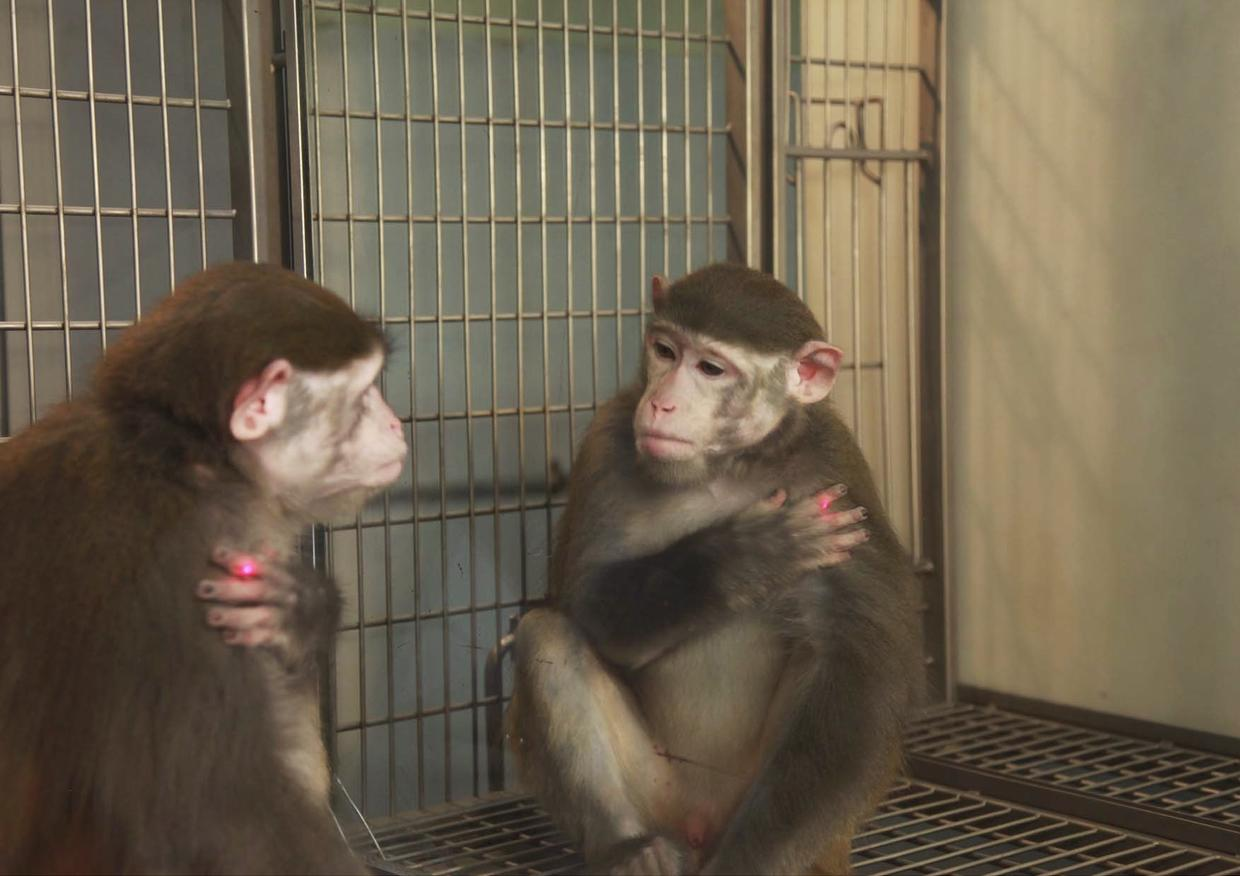
\includegraphics[width=\textwidth]{figures/mirror.jpg}
    \caption[As a component of the mirror test, a monkey observes its own reflection in the mirror
    ]{As a component of the mirror test, a monkey observes its own reflection in the mirror \citep{chang_mirror-induced_2015}.}
    \label{fig:mirror-test}
  \end{figure}

  Higher-order consciousness involves the awareness of being aware \citep{carruthers_higher-order_2020}, while global workspace consciousness represents the integration of information from various sources to tackle complex tasks \citep{baars_essential_1997}. Gaining a comprehensive understanding of these diverse forms of consciousness and other proposed classifications is essential for exploring the relationship between attention and conscious awareness.

  \subsection{Attention}
  \label{sec:attention}

  Attention is a core cognitive process that enables us to focus selectively on specific aspects of our environment while filtering out irrelevant stimuli. There are various types of attention, as shown in \autoref{tab:overview-attention}, with selective \citep{koivisto_relationship_2009} and divided attention \citep{mckanna_divided_2009} being two primary examples.

  In the context of consciousness, the previous chapter discussed various forms, such as phenomenal and access consciousness. Building on this understanding, selective attention can be linked to the cocktail party effect as originally published in the landmark paper from \cite{cherry_experiments_1953}, where people focus on a person’s voice in a crowded room while ignoring other conversations. This raises the question of the extent to which unattended information is processed within the scope of our conscious awareness.

  Conversely, divided attention allows simultaneous focus on multiple stimuli, like cooking while listening to a podcast. Research, like \cite{rodrigue_spatio-temporal_2015}, confirms successful dual-task performance under certain conditions.

  \vspace{10pt} % Increase vertical spacing before table
  \begin{table}[ht]
    \centering
    \renewcommand{\arraystretch}{1.5}
    \setlength{\tabcolsep}{12pt}
    \resizebox{\columnwidth}{!}{%
      \begin{tabular}{|>{\hspace{0pt}}m{0.18\linewidth}|>{\hspace{0pt}}m{0.78\linewidth}|} % adjust column widths
        \hline
        \rowcolor[HTML]{EFEFEF}
        {\color[HTML]{374151} \textbf{Types of \newline Attention}} & {\color[HTML]{374151} \textbf{Description}}                                                                                                     \\ \hline
        \rowcolor[HTML]{FFFFFF}
        {\color[HTML]{374151} Selective \newline Attention}         & {\color[HTML]{374151} This type of attention is characterised by the ability to focus on one particular stimulus while ignoring other stimuli.} \\ \hline
        \rowcolor[HTML]{FFFFFF}
        {\color[HTML]{374151} Divided \newline Attention}           & {\color[HTML]{374151} This type of attention involves the ability to attend to multiple stimuli at the same time without losing focus.}         \\ \hline
      \end{tabular}%
    }
    \caption{Types of attention and their descriptions.}
    \label{tab:overview-attention}
  \end{table}

  \subsection{Libet’s Delay}
  \label{sec:libet}

  In the previous chapter, the author discussed various forms of consciousness and the role of attention in shaping our conscious experiences. Another essential aspect of understanding the relationship between attention and consciousness is Libet’s delay. Libet’s original study involved participants voluntarily moving their fingers or hands and noting when they became aware of the intention to move \citep{libet_time_1983}. This delay, typically several hundred milliseconds as shown in \autoref{fig:libet-diagram}, has significant implications for understanding consciousness and its relationship to attention.

  \begin{figure}[ht]
    \centering
    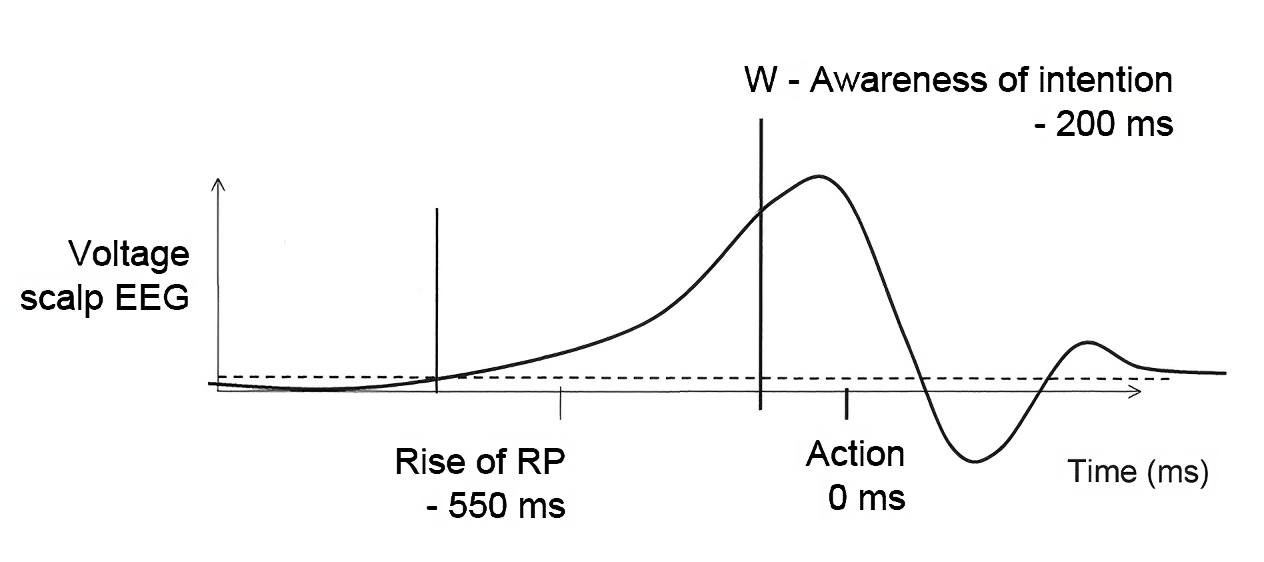
\includegraphics[width=\textwidth]{figures/libet.png}
    \caption[A diagram displaying the crucial characteristics of the outcomes obtained by Libet et al.]{A diagram displaying the crucial characteristics of the outcomes obtained by \cite{libet_time_1983} \citep{haggard_conscious_2001}.}
    \label{fig:libet-diagram}
  \end{figure}

  \newpage

  Libet’s delay indicates that subjective experience may not always align with actual neural processes, raising questions about attention’s role in shaping conscious experiences and adding temporal complexity to the attention-consciousness relationship \citep{dijksterhuis_goals_2010}. In the context of selective and divided attention, the delay’s impact on conscious awareness during these attentional states is worth considering.

  The influence of Libet’s delay on different forms of consciousness, such as phenomenal and access consciousness, should be contemplated. The temporal discrepancy may affect the relationship between attention and phenomenal consciousness differently than its relationship with access consciousness. Phenomenal consciousness might involve temporally separated subjective experiences, while access consciousness may be less affected by the delay, as information processing can occur independently of subjective experience \citep{dijksterhuis_goals_2010, kozuch_gorillas_2018}.

  \section{Attention’s Role in Conscious Awareness}
  \label{sec:evidence}

  \subsection{Empirical studies}
  \label{sec:empirical}

  Several empirical studies provide evidence for the link between attention and conscious awareness. One such study, conducted by \cite{cohen_attentional_2012}, investigated the attentional requirements of consciousness by manipulating the allocation of attention in a visual search task. As illustrated in \autoref{fig:cohen-attention} the authors found that when attention was directed away from a target stimulus, participants were less likely to report conscious awareness of the stimulus, suggesting that attention plays a critical role in conscious perception.

  \begin{figure}[ht]
    \centering
    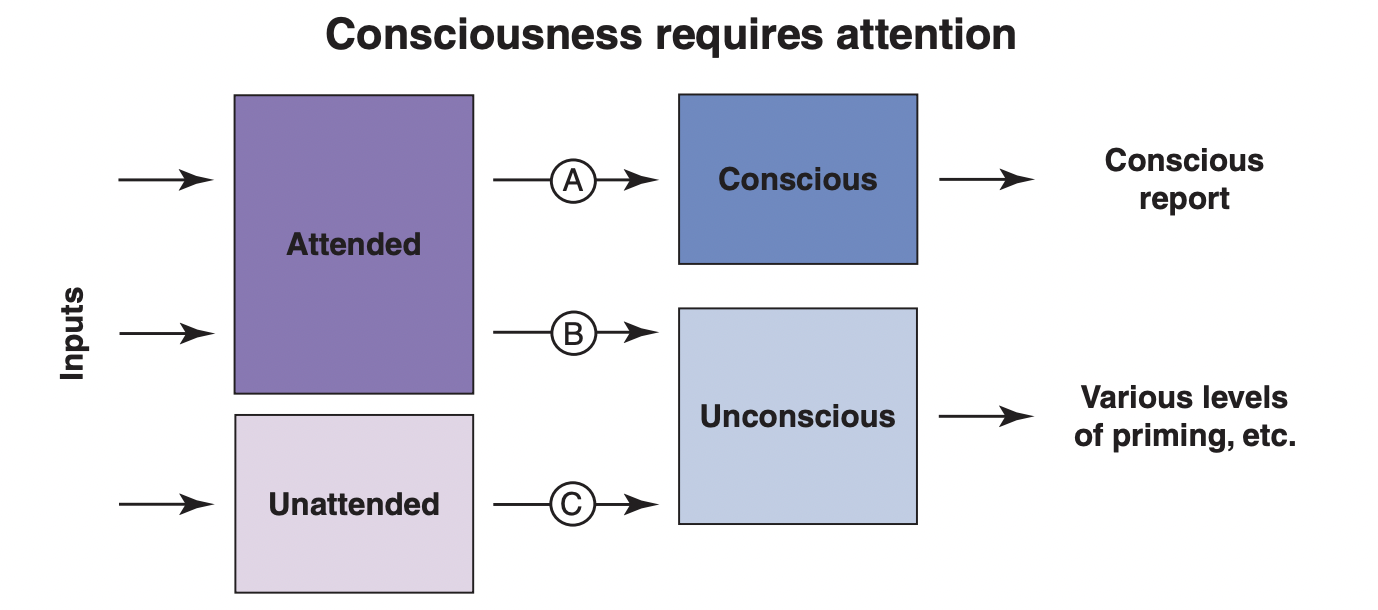
\includegraphics[width=\textwidth]{figures/attention.png}
    \caption[Explaining the link between attention and consciousness. According to the model, attention is necessary for information to become consciously aware, but not all attended stimuli will be perceived. Stimuli that are attended to but not perceived can still have measurable effects on behaviour and brain activity. Additionally, stimuli that are not attended to can still cause some neural activity, but the effects will be weaker.]{Explaining the link between attention and consciousness. According to the model, attention is necessary for information to become consciously aware, but not all attended stimuli will be perceived. Stimuli that are attended to but not perceived can still have measurable effects on behaviour and brain activity. Additionally, stimuli that are not attended to can still cause some neural activity, but the effects will be weaker \citep{cohen_attentional_2012}.}
    \label{fig:cohen-attention}
  \end{figure}

  Similarly, \cite{kentridge_spatial_2004} explored the role of attention in blindsight, a neurological condition in which individuals with damage to the primary visual cortex can respond to visual stimuli without conscious awareness. In their study, the authors demonstrated that when spatial attention was directed towards a stimulus, participants with blindsight exhibited faster response times, despite a lack of conscious awareness. This finding supports the idea that attention can influence unconscious processing and modulate conscious awareness.

  Another study by \cite{sumner_attentional_2006} investigated the role of attention in sensorimotor processes in the absence of perceptual awareness. The authors employed a visual masking paradigm to render stimuli imperceptible and found that attention could still modulate participants’ motor responses to the masked stimuli. This result implies that attention can modulate cognitive processes even when conscious awareness is absent, further highlighting the intricate relationship between attention and conscious awareness.

  \subsection{Theoretical perspectives}
  \label{sec:theoretical}

  Various theoretical perspectives also support the notion that attention is necessary for conscious awareness. \cite{baars_essential_1997} ’s Global Workspace Theory (GWT) positions that consciousness arises when information becomes globally available within the brain, and attention plays a crucial role in selecting and broadcasting this information. According to this theory, attention acts as a gatekeeper determining which information enters the global workspace and subsequently becomes part of our conscious experience as shown in \autoref{fig:workspace}.

  \begin{figure}[ht]
    \centering
    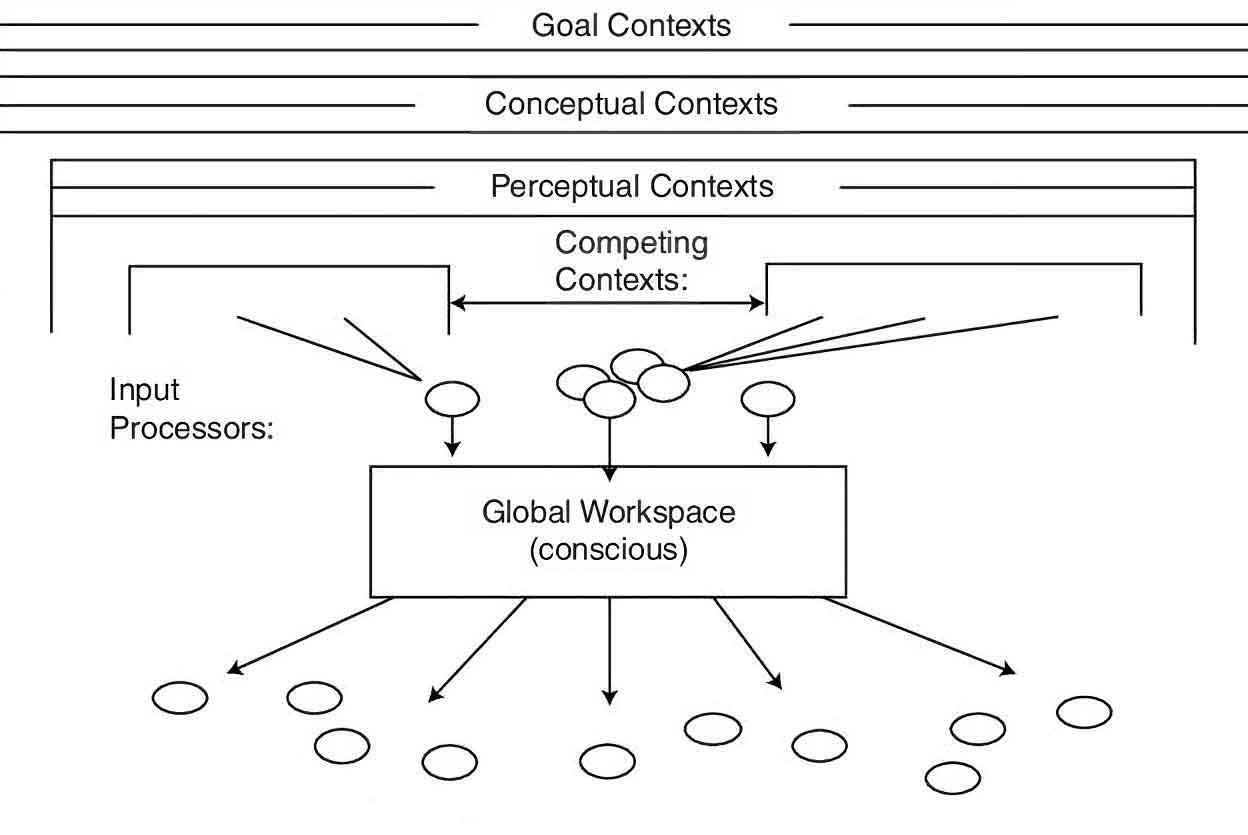
\includegraphics[width=\textwidth]{figures/global-workspace.jpg}
    \caption[Visualisation of Baars’ Global Workspace Theory.]{Visualisation of Baars’ Global Workspace Theory \citep{sun_computational_2007}.}
    \label{fig:workspace}
  \end{figure}

  \cite{de_brigard_role_2012} proposed an attentional relevance theory, suggesting that attention is necessary for the conscious recollection of past events. According to this theory, attention enhances the encoding and retrieval of memories by prioritising information relevant to our goals and interests. This perspective emphasises the role of attention in shaping the content of our conscious experiences, particularly in the domain of memory.

  Finally, \cite{dijksterhuis_goals_2010} put forth the idea that attention plays a crucial role in goal-directed behaviour, which is intimately linked to conscious awareness. The authors argue that attention activates and maintains cognitive representations of goals, enabling us to consciously pursue and achieve desired outcomes. This perspective highlights the importance of attention in bridging the gap between our conscious intentions and actions, further reinforcing the necessity of attention for conscious awareness.

  \subsection{Alternative viewpoints and evidence}
  \label{sec:alternative}

  While several studies support the necessity of attention for conscious awareness, others challenge this notion. \cite{aru_phenomenal_2013} summarised whether phenomenal awareness could emerge without attention using a visual paradigm in which participants reported their conscious experience of stimuli under various attentional manipulations. The authors found evidence for conscious perception even when attention was directed away from the target stimulus, suggesting that attention may not be strictly necessary for conscious awareness.

  \cite{kentridge_attended_2008} also questioned the sufficiency of attention for visual awareness, examining the interplay between attention and awareness in a patient with visual form agnosia, a condition characterised by the inability to recognise objects despite preserved low-level vision. The authors found that the patient could allocate attention to a stimulus without reporting conscious awareness of its shape or orientation, indicating that attention may be necessary but insufficient for visual awareness.

  Furthermore, \cite{kozuch_gorillas_2018} critically reevaluated the evidence that attention is necessary for consciousness, challenging the conclusions of several well-known studies, including the influential work by \cite{cohen_attentional_2012}. \citeauthor*{kozuch_gorillas_2018} argued that many studies supporting the necessity of attention for consciousness were methodologically flawed or misinterpreted, suggesting that the attention-consciousness relationship is still open to debate.

  Several theoretical perspectives and philosophical ideas propose alternative viewpoints on the attention-consciousness relationship. \cite{montemayor_types_2021} posited that consciousness encompasses multiple types, each with distinct neural correlates and functional roles. This perspective challenges the idea of a unified attention-consciousness relationship, suggesting that attention may differentially influence various types of consciousness.

  \cite{noah_recent_2020} presented a comprehensive review of recent evidence concerning the attention-consciousness relationship, concluding that while attention is necessary for conscious perception, it is insufficient. They argued that additional factors, such as the interaction between top-down and bottom-up processes, contribute to conscious awareness. This viewpoint highlights the complexity of the attention-consciousness relationship and encourages further exploration of the underlying cognitive and neural mechanisms. These alternative viewpoints and empirical findings demonstrate that the relationship between attention and conscious awareness is far from settled, inviting further investigation and debate.

  \section{Conclusion}
  \label{sec:conclusion}

  In this essay, the author critically evaluated the statement “attention is necessary for conscious awareness”, drawing upon diverse empirical and theoretical evidence. The essay began by defining the key concepts of consciousness and attention and highlighting their roles in cognitive phenomena. Additionally, it explored Libet’s delay and its potential implications for understanding the attention-consciousness relationship.

  Next, the author presented empirical studies supporting the necessity of attention for conscious awareness, demonstrating attention’s crucial role in shaping and modulating our conscious experience. However, the author also considered alternative viewpoints and evidence that challenge the necessity of attention for conscious awareness. The essay discussed studies offering alternative interpretations of the attention-consciousness relationship and contemporary theoretical perspectives that propose diverse and nuanced views on this relationship, such as those by \cite{montemayor_types_2021} and \cite{noah_recent_2020}.

  In conclusion, the relationship between attention and conscious awareness is complex and multifaceted, with Libet’s delay adding further intricacy. By examining diverse perspectives, we can enhance our understanding of the interplay between attention and consciousness while appreciating the dynamic nature of human cognition.

  \pagebreak
  \singlespacing % No need for double spacing in the references
  \bibliographystyle{references/custom-apa}
  \bibliography{references/bibliography}

\end{sloppypar}
\end{document}